\documentclass[letterpaper,landscape]{article}

\usepackage[margin=20mm]{geometry}
\usepackage{tikz}
\usepackage{graphicx}

\begin{document}
\thispagestyle{empty}
\begin{center}

{\Large\textbf{Print at EXACTLY 100\% scale. Do not "Fit to Page".}}\\
\vspace{2mm}
Cut along the outer black boundary (187.5\,mm\,$\times$\,142.0\,mm) and tape to the platform.\\
\textbf{Sheet 03: Mixed Colors \& Shapes}

\vspace{5mm}

\begin{tikzpicture}[x=1mm, y=1mm]

% 1. Draw the outer platform boundary (187.5mm wide, 142.0mm high)
% TikZ origin (0,0) is Top-Left. We draw downwards to match image coordinates.
\draw[thick] (0,0) rectangle (187.5, -142.0);

% 2. Place the 6 ArUco markers inset by 12mm from the edges.
% width=22.5mm so the inner black ArUco square is exactly 15mm.

% Top-Left (ID 0)
\node at (12, -12) {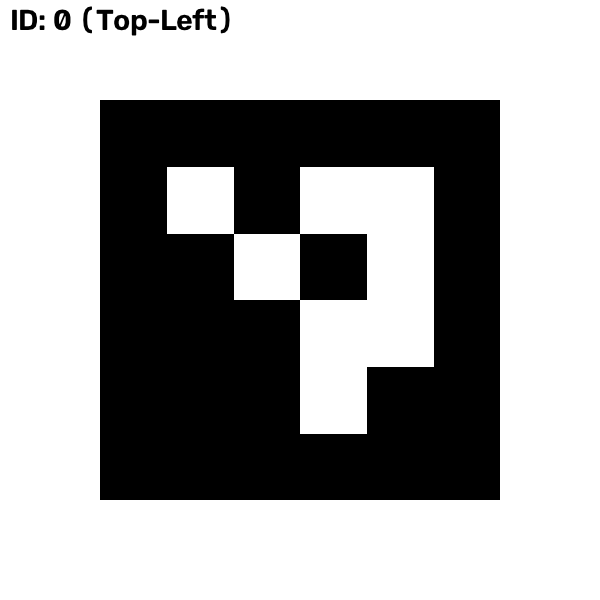
\includegraphics[width=22.5mm]{aruco/marker_0.png}};
% Top-Right (ID 1)
\node at (175.5, -12) {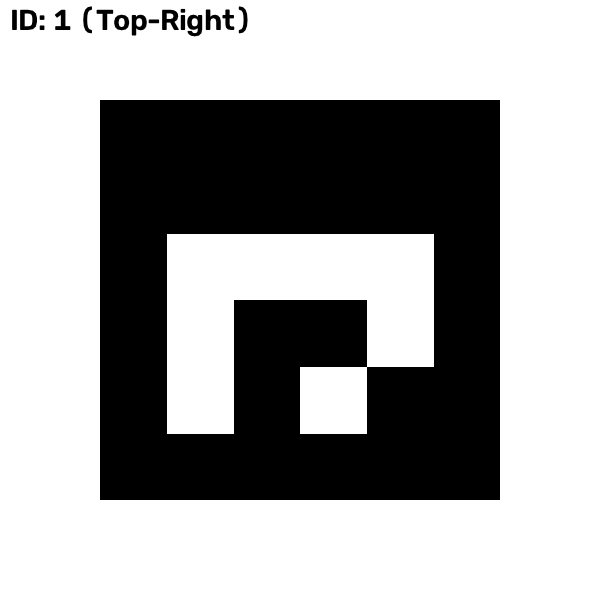
\includegraphics[width=22.5mm]{aruco/marker_1.png}};
% Bottom-Right (ID 2)
\node at (175.5, -130) {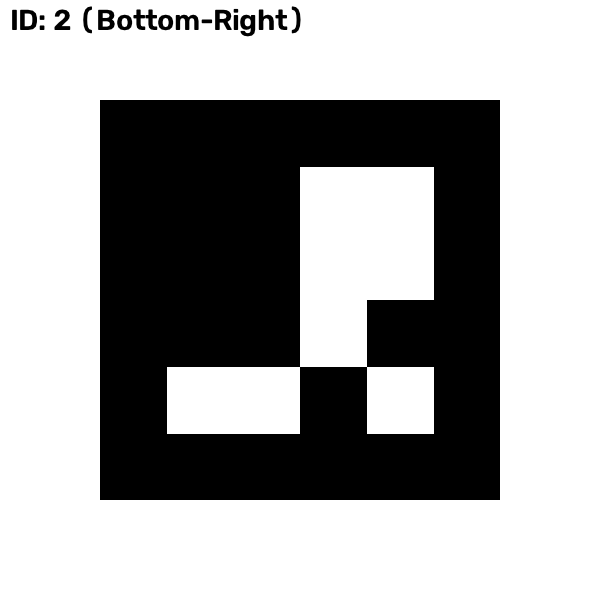
\includegraphics[width=22.5mm]{aruco/marker_2.png}};
% Bottom-Left (ID 3)
\node at (12, -130) {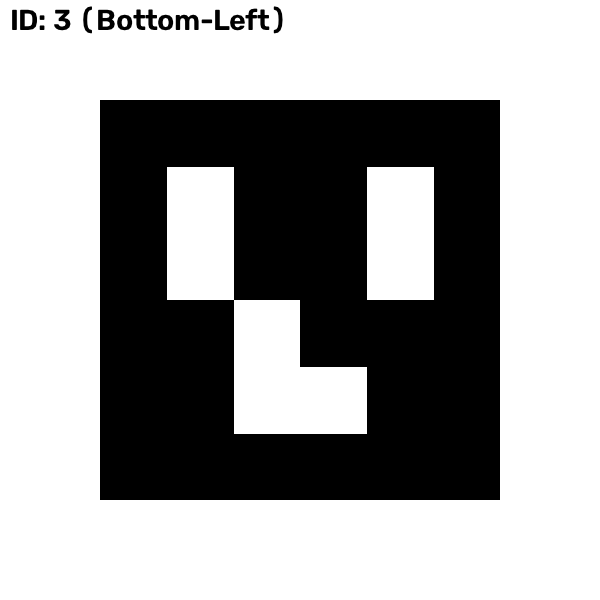
\includegraphics[width=22.5mm]{aruco/marker_3.png}};

% Middle-Left (ID 4)
\node at (12, -71) {
\includegraphics[width=22.5mm]{aruco/marker_4.png}};
% Middle-Right (ID 5)
\node at (175.5, -71) {
\includegraphics[width=22.5mm]{aruco/marker_5.png}};

% 3. Five mixed-color, mixed-shape features
% Arranged in a cross/quincunx pattern around center (93.75, -71)
% Spacing: ~30mm between shape centers
% All shapes inscribed within ~8mm effective radius

% Center - Black circle
\draw[fill=black, draw=black, thick] (93.75, -71) circle (8mm);

% Top - Blue triangle (pointing up)
\draw[fill=blue, draw=black, thick]
    (93.75, -41+9.24) -- (93.75-8, -41-4.62) -- (93.75+8, -41-4.62) -- cycle;

% Right - Yellow square
\draw[fill=yellow, draw=black, thick]
    (123.75-7, -71+7) rectangle (123.75+7, -71-7);

% Bottom - Green hexagon (regular, flat-top)
\draw[fill=green, draw=black, thick]
    (93.75+8, -101) -- (93.75+4, -101+6.93) -- (93.75-4, -101+6.93)
    -- (93.75-8, -101) -- (93.75-4, -101-6.93) -- (93.75+4, -101-6.93) -- cycle;

% Left - Red triangle (pointing up)
\draw[fill=red, draw=black, thick]
    (63.75, -71+9.24) -- (63.75-8, -71-4.62) -- (63.75+8, -71-4.62) -- cycle;

% 4. Dashed center crosshair for visual reference
\draw[gray, dashed] (93.75, -71) circle (3mm);
\draw[gray, dashed] (83.75, -71) -- (103.75, -71);
\draw[gray, dashed] (93.75, -61) -- (93.75, -81);

\end{tikzpicture}
\end{center}
\end{document}
